\documentclass[tikz,border=6pt]{standalone}
\usepackage{amsmath,amssymb}
\usepackage{xcolor}
\definecolor{accent}{HTML}{A13D2C}
\definecolor{accent2}{HTML}{2B5F6B}
\definecolor{muted}{HTML}{5A564F}
\definecolor{linecol}{HTML}{D8D2C4}
\definecolor{astroblue}{HTML}{1B4F72}
\usetikzlibrary{arrows.meta}
\usepackage[T1]{fontenc}\usepackage{newpxtext,newpxmath}  % same fonts as the notes
\begin{document}
% Intensity leaving a uniform slab of optical depth tau, I = I0 e^{-tau} + S (1 - e^{-tau}), with S = 1.
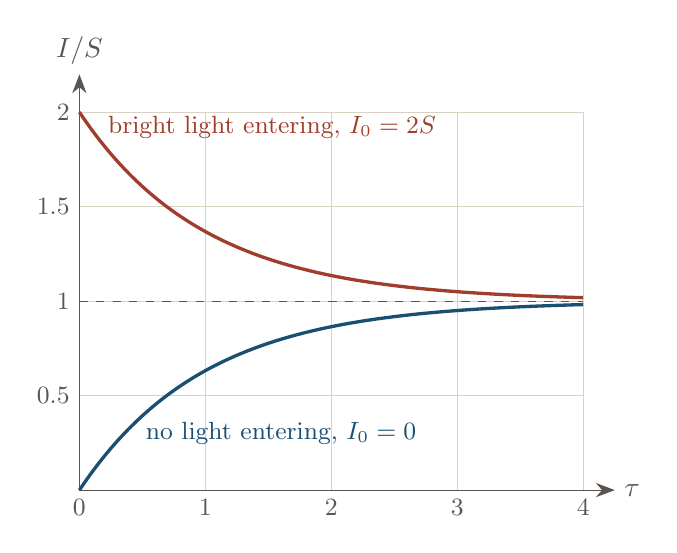
\begin{tikzpicture}[x=1.6cm,y=2.4cm, >={Stealth[length=2.4mm]}]
  \draw[linecol] (0,0) grid[xstep=1,ystep=0.5] (4,2);
  \draw[->, muted] (0,0) -- (4.25,0) node[right] {$\tau$};
  \draw[->, muted] (0,0) -- (0,2.2) node[above] {$I/S$};
  \foreach \x in {0,1,2,3,4} \node[below, muted] at (\x,0) {\small \x};
  \foreach \y in {0.5,1,1.5,2} \node[left, muted] at (0,\y) {\small \y};
  \draw[dashed, muted] (0,1) -- (4,1);
  \draw[accent, line width=1.2pt, domain=0:4, samples=100] plot (\x, {2*exp(-\x) + 1 - exp(-\x)});
  \draw[astroblue, line width=1.2pt, domain=0:4, samples=100] plot (\x, {0*exp(-\x) + 1 - exp(-\x)});
  \node[accent, right] at (0.15,1.92) {\small bright light entering, $I_0=2S$};
  \node[astroblue, right] at (0.45,0.3) {\small no light entering, $I_0=0$};
\end{tikzpicture}
\end{document}
